\documentclass[compress]{beamer}
%\documentclass[handout]{beamer}

\mode<presentation>
{
  \usetheme{CambridgeUS}      % or try Darmstadt, Madrid, Warsaw, ...
  \usecolortheme{default} % or try albatross, beaver, crane, ...
  \usefonttheme{default}  % or try serif, structurebold, ...
  \setbeamertemplate{navigation symbols}{}
  \mode<beamer>{\setbeamertemplate{blocks}[rounded][shadow=true]}
  \setbeamertemplate{caption}[numbered]
  \useoutertheme{infolines}
  \useoutertheme[subsection=false]{miniframes}
} 

\usepackage[english]{babel}
\usepackage[utf8x]{inputenc}
\usepackage{pifont}
\usepackage{amssymb}
\usepackage{xcolor}
\usepackage{tikz}
\newcommand{\xmark}{\ding{55}}%
\usepackage{eurosym}
\usepackage{graphicx}
% set colors
\definecolor{myNewColorA}{RGB}{0, 45,114}
\definecolor{myNewColorB}{RGB}{0, 45,114}
\definecolor{myNewColorC}{RGB}{0, 45,114} % {130,138,143}
\setbeamercolor*{palette primary}{bg=myNewColorC}
\setbeamercolor*{palette secondary}{bg=myNewColorB, fg = white}
\setbeamercolor*{palette tertiary}{bg=myNewColorA, fg = white}
\setbeamercolor*{titlelike}{fg=myNewColorA}
\setbeamercolor*{title}{bg=myNewColorA, fg = white}
\setbeamercolor*{item}{fg=myNewColorA}
\setbeamercolor*{caption name}{fg=myNewColorA}
\setbeamercolor{date in head/foot}{fg=white}
\setbeamercolor{page number in head/foot}{fg=white}


\titlegraphic{%
\vspace{0cm}
    \includegraphics[width=4cm]{logo-vertical2.png}
}

\usepackage{subcaption}
% \usepackage{mathrsfs}

\usepackage{dirtytalk}
\usepackage{tcolorbox}
\usepackage{multicol}
\usepackage{multirow}
\usepackage{caption}
\usepackage{threeparttable}
\usepackage{pdfpages}
\usepackage{longtable}
\usepackage{adjustbox}
\usepackage{colortbl}
\usepackage{tikz}
\def\checkmark{\tikz\fill[scale=0.4](0,.35) -- (.25,0) -- (1,.7) -- (.25,.15) -- cycle;} 
\usepackage{pdfpages}

\usepackage{accents}
\newcommand{\ubar}[1]{\underaccent{\bar}{#1}}
%\usepackage{enumitem}

%% References - BEGIN
\usepackage[backend=bibtex8,style=authoryear-icomp,doi=false,url=false,isbn=false,eprint=false]{biblatex}
\renewbibmacro{in:}{}		% gets rid of the 'In' in front of the journal name
%\bibliographystyle{natbib}        
% \bibliography{references.bib}

% diagram (tree)
\usepackage{tikz}
\tikzset{
  treenode/.style = {shape=rectangle, rounded corners,
                     draw, align=center,
                     top color=white,
                     bottom color=blue!20},
  root/.style     = {treenode, font=\Large,
                     bottom color=red!30},
  env/.style      = {treenode, font=\ttfamily\normalsize},
  dummy/.style    = {circle,draw}
}

\title{Elements of Microeconomics: \\
       Discussion Section 4} 
\author{Jamie Hyder}
\date{September 5, 2025}


\begin{document}

\begin{frame}
  \titlepage
\end{frame}

\begin{frame}{An opening question:}

\centering
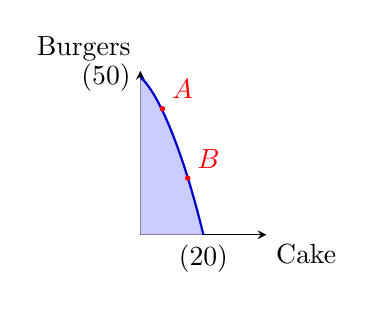
\begin{tikzpicture}[>=stealth, scale=0.04] % adjust scale for slide fit
  % Axes
  \draw[->] (0,0) -- (40,0) node[below right] {Cake};
  \draw[->] (0,0) -- (0,52) node[above left] {Burgers};

  % Feasible region shading (light blue)
  \begin{scope}
    \path[clip] (0,50) .. controls (6,45) and (14,25) .. (20,0) -- (0,0) -- cycle;
    \fill[blue!20] (0,0) rectangle (22,52);
  \end{scope}

  % PPF curve (dark blue, concave to origin)
  \draw[thick, blue!80!black]
    (0,50) .. controls (6,45) and (14,25) .. (20,0);

  % Intercept labels
  \node[left]  at (0,50) {(50)};
  \node[below] at (20,0) {(20)};

  % Efficient points on the PPF
  \fill[red] (7,40) circle (25pt) node[above right] {$A$};
  \fill[red] (15,18) circle (25pt) node[above right] {$B$};
\end{tikzpicture}


\begin{block}{A restaurant produces burgers and cake, and needs to split their resources/inputs among production of the two goods...}
Points A and B on the graph represent the production quantities:
    \begin{itemize}
        \item A: 7 cakes and 40 burgers
        \item B: 15 cakes and 18 burgers
    \end{itemize}
\textbf{What is the opportunity cost of moving from point A to point B in terms of cake?}\textit{ (ie for each additional burger how much cake must we give up)}
\end{block}

\end{frame}    



% Outline frame
\begin{frame}{Outline - CH 3: "Interdependence and the Gains from Trade"}

    The main takeaways from this chapter are on \textbf{\textit{advantage}} --- both \textit{absolute and comparative} --- and the benefits of specialization and trade.
\end{frame}

\begin{frame}{Thinking at the margin}
Something we glossed over in last week's discussion:

\begin{block}{}
    \begin{center}
        \textit{Economists think at the margin.}
    \end{center}
\end{block}

    More importantly, we believe that \textbf{firms and individuals do the same.
}
    \medskip
    \medskip

    This means when evaluating a decision, we think about what a small change in behavior will do to an outcome.

\end{frame}

% How people make decisions
\begin{frame}{Absolute advantage}
\begin{block}{}
    \textit{Absolute advantage} describes the ability to produce more of a good given a fixed quantity of inputs.
\end{block}
    \medskip

Let's consider two restaurants: Muffin's Steakhouse and Sandy's Salads. Both of them can produce two dishes: salads and steaks. Given 1000 minutes of labor time, they can produce the following amounts of each dish:

    \begin{table}[h]
  \centering
  \begin{tabular}{|c|c|c|}
    \hline
    \textbf{Restaurant} & \textbf{Steaks} & \textbf{Salads} \\
    \hline
    \textbf{Muffin's Steakhouse} & 100 & 20 \\
    \hline
    \textbf{Sandy's Salads} & 200 & 100 \\
    \hline
  \end{tabular}
  \caption{Muffin vs. Sandy}
\end{table}

    What is their cost, in minutes, to produce steak and salads?
\end{frame} 

\begin{frame}{Absolute advantage}
    Assume that there is a \textit{constant transferability} from one dish to the other:
    \begin{enumerate}
        \item Draw the production possibility frontiers for the two restaurants.
        \item Who has the absolute advantage in producing steaks?
        \item Who has the absolute advantage in producing salads?
    \end{enumerate}

\vfill
\begin{center}
    \includegraphics[width=0.25\linewidth]{Sandy Chef.png} \hspace{1em}
    \includegraphics[width=0.25\linewidth]{Muffin Chef.png}
\end{center}
\end{frame}

\begin{frame}{Comparative advantage}
   Before we discuss comparative advantage, let's think about the opportunity cost of each firm for each dish:
   \begin{enumerate}
    \item What are the slopes of the two PPFs?
    \item What is Muffin's opportunity cost for producing steaks and salads?
    \item What is Sandy's opportunity cost for producing steaks and salads?
   \end{enumerate}
   In other words: what is the \textit{trade-off} that each restaurant faces as they change their production from one dish to another?
\end{frame} 

\begin{frame}{Comparative advantage}
    The \textit{opportunity cost} of producing salads is the amount of steaks they could have produced with the same input. In our example, this is constant.

    \medskip
    
\begin{block}{}
    A restaurant has a \textit{comparative advantage} in producing steaks compared to their competitor if their opportunity cost is lower.
\end{block}

    \medskip

    \begin{enumerate}
        \item Can a firm have an absolute advantage in both goods?
        \item Can a firm have a comparative advantage in both goods?
        \item What is the relationship between the comparative advantage in good A and good B?
    \end{enumerate}
\end{frame} 

\begin{frame}{Comparative advantage}
\begin{itemize}
    \item   The comparative advantage in producing good A is the \textit{inverse} of the comparative advantage in producing good B.
    \item     If the comparative advantage in good A is high, the comparative advantage for good B must be low.

\end{itemize}

    \medskip

    Comparative advantage depends on the \textit{opportunity cost}: these concepts are linked.
\end{frame} 

\begin{frame}{Comparative advantage}
    Since most customers like to order a salad with their steak, Sandy and Muffin both want to offer both salads and steaks (not necessarily in equal quantities).

    \medskip

    If both spend half their resources on each dish, what is their output?

    \medskip

    Now suppose the two restaurants can trade with each other. What is one set of productions, and one possible trade, which would leave them both better off?

\end{frame} 

\begin{frame}{Comparative advantage}
    When they both split their 1000 minutes 50/50 between the two dishes, their output is:

    \begin{table}
    \begin{tabular}{|c|c|c|}
      \hline
      \textbf{Restaurant} & \textbf{Steaks} & \textbf{Salads} \\
      \hline
      \textbf{Muffin's Steakhouse} & 50 & 10 \\
      \hline
      \textbf{Sandy's Salads} & 100 & 50 \\
      \hline
      \textbf{Total output} & 150 & 60 \\
      \hline
    \end{tabular}
    \caption{50/50 split}
  \end{table}

\end{frame} 

\begin{frame}{Possible trade}
    There are many possible answers to this last question, but let's go back to our principle at the beginning of the discussion, and \textit{think at the margin}.
    \begin{itemize}
        \item Muffin produces 1 fewer salads and 5 more steaks
        \item Sandy produces 2 fewer steaks, and 1 more salad
    \end{itemize}
    Then their production is:

    \begin{table}
    \begin{tabular}{|c|c|c|}
      \hline
      \textbf{Restaurant} & \textbf{Steaks} & \textbf{Salads} \\
      \hline
      \textbf{Muffin's Steakhouse} & 55 & 9 \\
      \hline
      \textbf{Sandy's Salads} & 98 & 51 \\
      \hline
      \textbf{Total output} & 153 & 60 \\
      \hline
    \end{tabular}
    \caption{Possible trade}
  \end{table}

    Total production has gone up!
\end{frame} 

\begin{frame}{Possible trade}
    Which trade would leave them both better off?

    \medskip

    Say Muffin trades 3 steaks to Sandy in exchange for one salad:

    \begin{table}
    \begin{tabular}{|c|c|c|}
      \hline
      \textbf{Restaurant} & \textbf{Steaks} & \textbf{Salads} \\
      \hline
      \textbf{Muffin's Steakhouse} & 52 & 10 \\
      \hline
      \textbf{Sandy's Salads} & 101 & 50 \\
      \hline
    \end{tabular}
    \caption{Gains of trade}
  \end{table}

    They both have the same amount of salads as before, but more steaks! So we can say that they are each better off.

    \medskip
    
    Should they continue to specialize?

\end{frame} 

\begin{frame}{Price of trade}
    Here we just asserted a trade that would make both parties better off in terms of the amount of each dish. But how can we know both parties will agree to the trade?
    
    \medskip

    This is determined by the price of each good. In the example we gave, the ``price'' of one salad was 3 steaks.

    \begin{enumerate}
        \item What if the price of 1 salad was 3.5 steaks?
        \item What if the price of 1 salad was 1 steak?
        \item What if the price of 1 salad was 6 steaks?
    \end{enumerate}
\end{frame}

\begin{frame}{Price of trade}
    The first example would still leave both parties better off, but the second two would not.

    \medskip

    We are not ready yet to discuss where prices come from, but we do have a general rule:

    \begin{center}
        \textit{For trade to make both parties better off, the price must lie between the two opportunity costs.}
    \end{center}

\end{frame}

\begin{frame}{Discussion questions}

\begin{enumerate}
    \item Should Kevin Durant wash his own car?
    \item Should the U.S. trade with other countries?
    \item Should a chef build his own house?
    \item Should I make my own clothes?
    \item Should you be teaching this class?
\end{enumerate}

    \medskip

    \begin{block}{The main takeaway from this chapter:}
        \textit{Due to comparative advantage, specialization and trade can leave everyone participating better off.}
    \end{block}

\end{frame} 


\end{document}
     


